\chapter{Identifying Weakly Connected Subsystems in Building Energy Model (BEM) for Effective Load Estimation}
\label{chap:building}

\section{Introduction}
In 2016, the building sector used approximately 40\% of the energy produced in the United States~\citep{useia2017}, and in 2009, buildings contributed 2,184.6 million metric tons of carbon dioxide equivalent of greenhouse gases due to emissions~\citep{useia2009}.  As a result, governments and municipalities have committed to reducing the energy consumption of buildings.  New York State, for example, enacted Executive Order 88, which requires government buildings to reduce energy consumption by 20\% \citep{statedirect}, and the Public Service Commission in New York has established a public fund to target energy efficiency measures~\citep{nyspublic}. 

It is necessary to estimate the expected energy usage of a building to determine how to reduce energy usage. The expected energy usage of a building can be faithfully simulated using a Building Energy Model (BEM). Currently, there are several popular options for software to estimate the dynamic energy use, such as EnergyPlus, eQUEST, TRACE 700, and Carrier HAP~\citep{Eplus,hirsch2006equest, trace, HAP}, each of which utilizes a complex algorithm, built upon the heat-balance method, to calculate building loads. The BEMs incorporate energy load estimation due to the presence of HVAC systems, lights, and receptacle loads, and requires a substantial number of input parameters.   

Many of the numerous input parameters in a BEM are uncertain.  Some of these parameters are measured, while the owner, designer, or modeling professional must estimate others, and some are assumed by the BEM itself.  In each case, uncertainty is brought into the modeling results.  These uncertainties in the BEM can be categorized into two types: uncertainties in the measured parameters and the uncertainty in modeling~\citep{ding2015uncertainty,sun2015quantification}. To ensure that the building simulation is sufficiently accurate, and to better understand the impact of imprecisions in the input parameters and calculation methods, it is desirable to quantify uncertainty in the BEM throughout the modeling process. Uncertainty quantification (UQ) typically requires a large number of simulations to produce meaningful data, which, due to the vast number of input parameters and the dynamic nature of building simulation, is computationally expensive~\citep{rysanek2013optimum,eisenhower2012uncertainty}. We must, therefore, UQ in BEMs to a less computationally expensive model.

To enable computationally efficient UQ of BEM, following main contributions are made in this chapter:

\begin{itemize}
\item Adaptation of lumped resistor-capacitance network model to generate reduced order differential equation for BEM simulation
\item Usage of a gray-box method in conjunction with black-box Kalman filter to enable BEM parameter estimation
\item Application of WCSs identification-based UQ framework developed in Chapter~\ref{chap:wcs} to propagate the quantifiable uncertainty in the BEM.
\end{itemize}

Next, all the three main contributions are further elaborated.

The well-established technique of a lumped resistor-capacitor network is used to calculate the reduced-order zone heat balance equations. The RC method assumes that the components of the zone load can be estimated by a discrete number of resistances and capacitances, and the system is treated as equivalent to an electrical circuit~\citep{vivian2017evaluation}. In particular, the heat transfer due to the zone envelope can be reduced to a three resistance, two capacitance (3R2C) thermal network. With the RC network, one can reduce the load calculations to first-order differential equations that provide a suitable framework to carry out UQ in BEMs. 

The BEM simulation can be carried out using one of the three main models~\citep{he2016simplified,perera2014modeling}:

\begin{enumerate}
\item \textit{White box models:} In white box models detailed information about the known physical process is used to predict the future states.
\item \textit{Black-box models:} In black-box models measured data is used to estimate non-physical parameters that abstractly represent the BEM performance.
\item \textit{Gray-box models:} Gray-box models combine both the white-box and black-box methods through the use of a reduced order model with known building properties for modeling the physical process. Such models can also be easily combined with Kalman filtering to enable parameter estimation. Usage of gray-box models reduces computation time while improving the accuracy of predictions.
\end{enumerate}

Because of a large number of input parameters, despite the use of reduced order model, the resulting filtering problem is computationally expensive. The novel method of identifying Weakly Connected Subsystems (WCSs)~\citep{mukherjee2015laplacian,mukherjee2015non} is used to address this problem of performing UQ in the BEM. WCS-based UQ approach allows us to group coupled parameters to minimize the associated computation time required while continuing to propagate the quantifiable uncertainty present in the BEM. The overall approach is described in detail (later in this chapter). The optimal estimation problem to estimate parameters for UQ of BEM is the heart of this chapter.

A representative case study, a well-documented building, located in Central New York is used for modeling purposes. The created simulated model of the represented building allows us to treat many of the inputs as known parameters, with some initial uncertainty. 
%Internal loads, however, such as occupancy and receptacle loads, are difficult to assume with accuracy, as explained later in this work, so we use the measured data in an optimization routine to estimate the values.  Similarly, solar radiation is not measured in real time at the building site and can be loosely calculated based on historical solar data, but for accuracy, solar heat gain is also a good candidate for parameter estimation.
A reduced order model with a robust parameter estimation tool allows us to enable Model Predictive Control (MPC).  With MPC, the measured states of the building are used in conjunction with the predictive model.  At each sampling interval, the program performs an optimization algorithm to determine how the HVAC system should respond to the current building conditions~\citep{kelman2013analysis}.
%In this work, we investigate treating the supply air temperatures delivered by the HVAC system as unknown, and use the optimal estimation method to determine the required fan-coil output temperatures.

\section{Related Works}
\label{literature}
\subsection{Lumped capacitance RC network }
The lumped capacitance RC network reduced-order model method has been reliably used in a diverse assortment of research work to estimate the heat transfer due to the building envelope ~\citep{ramallo2013lumped,vsiroky2011experimental,li2017development}.  Further precision has been incorporated into the RC network by using dynamically estimated capacitances ~\citep{jara2016new} and second-order thermal network models ~\citep{underwood2014improved}.  The physics-based Three resistor-Two Capacitance (3R2C) model has been shown to be sufficiently accurate for approximating building models ~\citep{kircher2015lumped} based on parameters with physical meaning. In the outlined work, 3R2C models are used for modeling purpose.

Expanding the scope of the RC method, the lumped capacitance method has been used to estimate other factors affecting the thermal zone heating and cooling requirements.  The thermal mass of the zone, in particular, can be modeled with an RC network ~\citep{perera2014modeling,wang2006parameter}.  When these values are significant, long-wave radiation ~\citep{he2016simplified} and convective heat between zones ~\citep{goyal2011identification} can be modeled as black-box data-driven estimations.  Internal loads, especially, have been estimated using a filtering method in conjunction with the RC method for the surfaces ~\citep{o2010model}.

The existing literature related to the RC method are inadequate for modeling large-scale problems due to high computational cost. This computational cost is exacerbated due to increase in the number of inputs. Thus, a key contribution is in the development of a computational method to expedite the UQ using the idea of \textit{divide and conquer}.  


\subsection{Uncertainty Quantification in BEMs}

Uncertainty Quantification (UQ) is becoming more prevalent in the BEM domain, as building simulation software and methods continue to evolve~\citep{woloszyn2017treating}. Research in the field of UQ in BEM is growing at a fast pace. As explained earlier, uncertainty in a BEM can arise due to the modeling process or uncertainty in the parameters. All BEMs necessarily make assumptions to simplify the modeled building. Simplifying the assumptions in the building energy simulation domain causes the associated uncertainty to be often ignored. Few works have focused on quantifying the uncertainty in the actual modeling process. For example Sun et al.~\citep{sun2015quantification} have focused on incorporating the uncertainty in the actual in solar irradiation calculation and its effects on the results of BEM simulation. Additionally post-processing techniques have been developed for incorporating UQ in BEMs~\citep{ding2015uncertainty}. 

Recent studies used parameter estimation for UQ in BEMs. Both physics-based and surrogate models have been studied to optimize building performance under uncertainties by simulation methods~\citep{nguyen2014review}. It has been shown that even moderately variable parameters can have a significant effect on the overall BEM uncertainty, especially, when the small scale models are combined to generate a large-scale BEM, as demonstrated in multi-building residential district models~\citep{kavgic2015application,baetens2016modelling}.  Sensitivity analysis has often been used to determine the impact of uncertainty in parameters on the performance of the building energy model~\citep{rodriguez2013uncertainties,tian2013review}. Most of the work in sensitivity analysis focuses on identifying few most important parameters that can be used for further investigation during UQ. Additionally, most of the reported works are often limited to evaluating only particular aspects of a building and not the whole building~\citep{baetens2016modelling}. %In the case of unknown economic conditions, non-probabilistic criteria have been used to optimize uncertainty in the building ~\citep{rysanek2013optimum}. 


UQ in BEMs is also performed in Stochastic Model Predictive Control (SMPC) frameworks that utilize the dynamic state-space equations. Oldewurtel et al. have discussed how SMPC framework can be used to account for the uncertainty in weather predictions for building energy modeling purposes~\citep{oldewurtel2012use}. In related another work a SPMC has been developed to optimize building energy usage and has been shown to outperform existing Rule-based Control (RBC)~\citep{oldewurtel2010energy} framework. SPMC has also been used for large-scale building (large number of state variables) in the presence of uncertainties in weather prediction~\citep{oldewurtel2014stochastic}. Privara et al.~\citep{privara2011model} have used an identified state-space model of a real building to estimate the optimal energy consumption. The model developed by Privara et al. does not include the effect of internal loads or solar gains. An adaptive MPC has been developed incorporating uncertainties in a wide range of parameters including building materials, their thermal properties, and HVAC parameters~\citep{kim2013building}.

%Ma et al~\citep{ma2012model} discusses how a control input cost and a constraint violation are computed in a closed loop for a building in California using the state-space equation. Based on the efficiency obtained from this calculation, thermal load profiles are estimated. This method provides for a simple and computationally efficient way of calculating the uncertainty in a model. Although, the accuracy and scalability of this method are questionable. Siroky et al.~\citep{vsiroky2011experimental}

%When determining the model parameters to be used in RC networks, a bevy of methods can be applied. Siroky et al. outline two possible methods~\citep{vsiroky2011experimental}. Either the construction plan can be used to determine the unknown parameters, or they can be determined via statistical estimation.Statistical estimation methods are used so that the noise associated with the measurements are taken into account. 

%Li et al. employed Genetic Algorithm to search for the most optimal parameters to identify the model parameters utilized in their star-type RC model~\citep{li2017development}. Agbi et al. developed an algorithm to determine the numerical identifiability for high order RC models ~\citep{agbi2012parameter}. The algorithm is a closed loop “active-identification” architecture that improves experimental design for better data. It is shown that the algorithm useful since they can reduce disturbances to a minimum for building models.

%Also, some researchers determined what their model input parameters are so that their models could be simplified. Liao et al. propose a simplified physical model to estimate average air temperature in multi-zone heating systems ~\citep{liao2004simplified}. The model can achieve long-term accuracy and is also simple to manufacture and employ. The model has three input parameters: fuel consumption, external temperature, and solar radiation.

%All of these different methods are similar to those used in this work, but this work determines input parameters by way of the building documentation while also using a more scalable algorithm to propagate uncertainties in the input parameters.

   
A simulation over an extensive range of values is required with a minimum computational expense to enable UQ.  To reduce the computation time, techniques such as quasi-random sampling ~\citep{eisenhower2012uncertainty} and pre-processing historical data in modeling predictive controls~\citep{maasoumy2014handling} have been used. Similarly, other sampling-based methods or quadrature-based methods can also be applied (Chapter~\ref{chap:uq}). When applied to large scale problems with many input parameters, the performance of existing methods are computationally inefficient. To significantly improve the computational efficiency of UQ methods for quantification of uncertainties in large scale BEMs, the Weakly Connected Subsystems based UQ method ~\citep{Mukherjee_2017,mukherjee2015non,mukherjee2015laplacian}, that uses a clustering algorithm to enable a divide and conquer approach is used.



\section{Methodology}

\subsection{Proposed Framework}

In this section, the critical components for the UQ and optimal load estimation in BEM simulation have been outlined. Figure~\ref{fig:bem_framework} depicts the overall UQ framework for a large-scale BEM. Given an office/school building (Figure~\ref{fig:bem_framework}(a)), the geometry and the thermal properties of the building  are assessed to formulate the state-space equation model of a dynamical system ((Figure~\ref{fig:bem_framework}(c))). This state-space equation is formulated using the concept of RC network ((Figure~\ref{fig:bem_framework}(b))). The output equation is framed depending on the available measurement. A graph-theoretic representation is adopted to model the thermal network as an undirected graph ((Figure~\ref{fig:bem_framework}(d))). The state-space equation and the initial uncertainty information is used to quantify the adjacency information for the undirected graph (Figure~\ref{fig:bem_framework}(e)). A suitable graph clustering algorithm (Louvain modularity optimization) is then implemented to identify the Weakly Connected Subsystems or WCSs (Figure~\ref{fig:bem_framework}(f)). Subsequently, the input formulation involving the weather (ambient temperature), the HVAC (airflow), and soil temperature are obtained, and the solar gain for the exterior walls are calculated ((Figure~\ref{fig:bem_framework}(g))). The statistical properties of the state variables are propagated through each WCSs, which are updated based on the measurement availability. The updated statistical properties give us the estimated parameters such as internal load, the solar gain for internal walls, along with the zonal temperatures, and the wall surface temperatures. In the subsequent sections, the individual components of the overall framework are described in details. 

\begin{figure}[H]
\centering
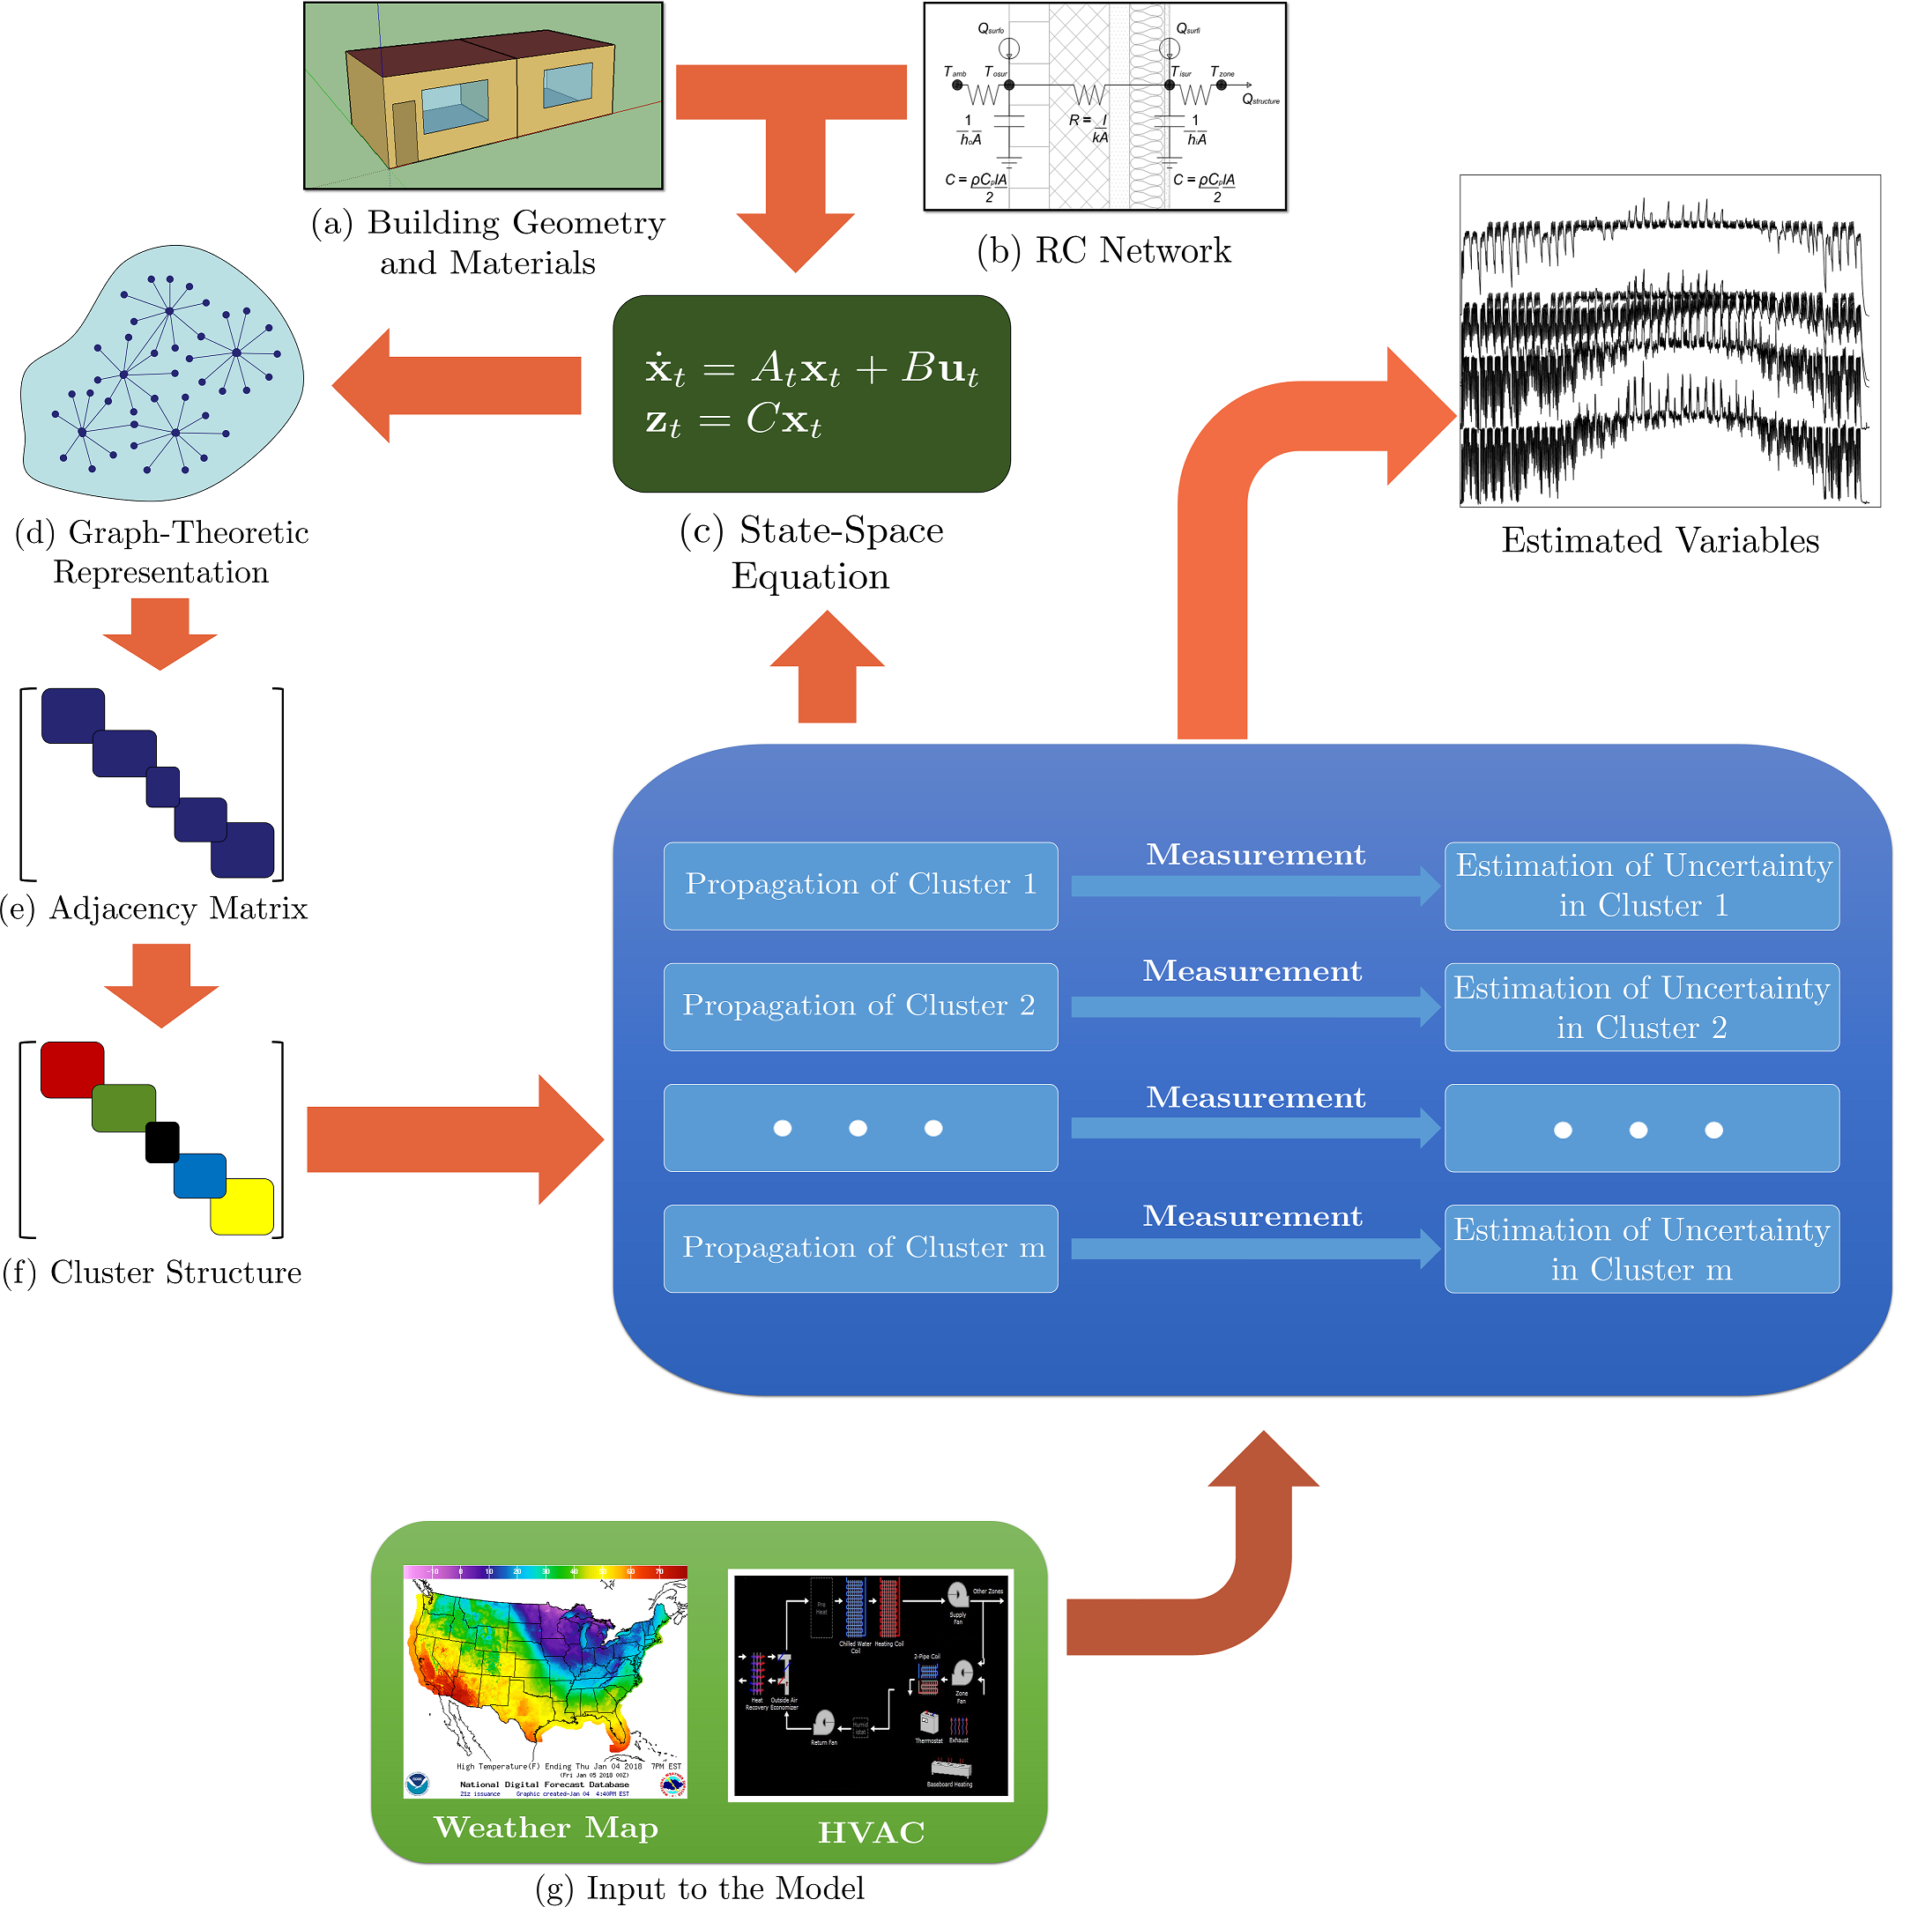
\includegraphics[width=\textwidth]{jbs_figures/bem_framework}
\caption{Schematic of the WCS identification-based UQ to estimate thermal load in a large-scale BEM. Weather Map~\citep{weathermap}}
\label{fig:bem_framework}
\end{figure}

\subsection{Materials and Geometry}
\label{MatGeo}

In order to perform a simulation with a BEM, the building geometry and surface properties must first be determined.  The building is divided into thermal zones, based upon the actual HVAC system; each area with an individual temperature sensor is a thermal zone.  Within the zone, the surfaces are determined, including the surface type (exterior, interior, or underground), the orientation, any adjacent zone information, and the surface dimensions.  Windows are located on the surfaces as well, and the area and any shading devices are noted.  These surfaces are critically important for the BEM, since the heat transfer occurring through the surfaces is a fundamental concept for these calculations.  Boundary conditions and orientation, in particular, determine the extent that the ambient temperature and solar effects impact the zone.  

For each surface, the material properties are determined, in order to calculate the thermal resistance and capacitance necessary for the RC network methodology.  Thermal resistance is calculated using the material thickness $l$ and conductivity $k$, and is a measurement of the heat flow across a surface at steady state conditions ~\citep{american90}.  Heat capacitance indicates the amount of heat input required to raise the temperature of a material, which demonstrates the capability of a material to store heat and delay heat transfer across the material, and is otherwise known as thermal mass ~\citep{american90}.  Capacitance can be likewise calculated using the material thickness $l$, density $\rho$, and specific heat $C_p$.  In order to obtain the overall surface properties, all materials in the surface construction must be combined; both resistance and capacitance can be treated as a circuit in parallel.

The values of the material properties are determined by testing.  In a building, the properties are assumed based upon either specific data published from the manufacturer, or, if unknown, typical values of materials are compiled in subject references \citep{american20132013}.  In some cases, values of typical wall constructions as a whole are published. 

\subsection{RC network}
\label{building_method}

As explained previously, the resistor-capacitor estimation method reduces the building surfaces into a discrete number of resistances and capacitances.  A three resistance, two capacitance model (3R2C) is the most used.  The used model for thermal load estimation model has been found to estimate the effects of the building surfaces on a thermal zone with sufficient accuracy~\citep{kircher2015lumped}.  Using this method, the heat balance equation can be broken into distinct parts that enables us to perform the load optimization.  The RC network for the surface constructions used for modeling purposes is shown in Figure~\ref{rc_walls}.

\begin{figure}[H]
\centering
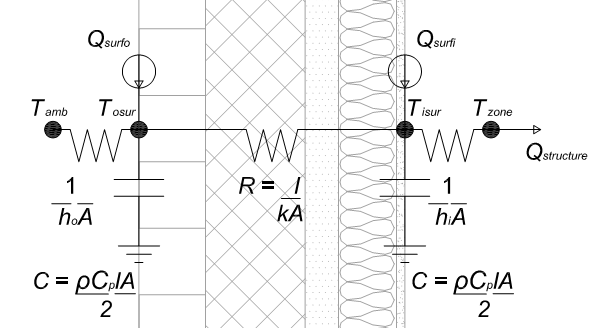
\includegraphics[scale=0.4]{jbs_figures/RC}
\caption{RC network for surface constructions}
\label{rc_walls}
\end{figure}

For most of the input parameters in the BEM, because of the extensive building documentation, physical data of the building is used for modeling purposes. Each of the known parameters has uncertainty associated with it that can be propagated through the BEM. Material properties are obtained from manufacturer’s literature, if known, or typical values based on testing ~\citep{american20132013}. The surface conductances, $h_{o}$ and $h_{i}$ are assumed to be static based on surface location and position~\citep{kircher2015lumped}.  Windows are assumed to be resistance-only constructions (1R) and thus are assumed to have no thermal mass. Due to the properties of glass and the small thickness, any effect due to thermal capacitance of windows is negligible. The glazing of windows can be modeled using only the specified resistance~\citep{kircher2015lumped}.

For interior zones, the adjacent zone temperature $T_{out}$ is a state variable. For exterior walls, the $T_{out}$ is the outdoor air temperature $T_{amb}$ that is available from weather data. Like the majority of building modeling techniques, the air in the zone is assumed to be well-mixed~\citep{fisher1997convective}. Thus, the variation of the zonal temperature $T_k$ with space is zero. Similarly, uniform surface temperatures and irradiation, diffuse radiating surfaces, and one-dimensional heat conduction are assumed through the assembly of multiple construction layers~\citep{american20132013}.

Given these assumptions, the BEM problem is simplified into a linear heat balance equation, with supply and return/relief airflows balance as follows~\citep{doe2016energyplus}:

\begin{equation}
\label{heat_balance}
\resizebox{0.9\textwidth}{!}{$
\displaystyle C_z \frac{dT_i}{dt} = \sum_{i} \dot{Q} + \sum_i h_i A_i (T_{sl} - T_z) + \sum_i \dot{m}_i C_p (T_{zi} - T_z) + \dot{m}_{inf}C_p(T_{\infty} - T_z) + \dot{m}_{sys}C_p (T_{sup} - T_z)
$}
\end{equation}

The definitions of the Solar Heat Gains $U_o$ and $T_q$ are discussed later. This equation states that the energy stored in the zone air is equal to the sum of the convective internal loads, the convective heat transfer from the zone surfaces, the heat transfer due to inter-zone air mixing, the heat transfer due to infiltration of outside air, and the heat transfer due to the output of the HVAC system into the zone.
Latent loads are ignored in the BEM, since humidity is not directly controlled, and is handled as a side-effect of the sensible cooling.  Humidity primarily affects occupant comfort, although a small amount of heat transfer occurs due to moisture in the air, with minimal impact on the zonal temperatures ~\citep{american20132013}.  Long-wave radiation exchanges between surfaces are ignored as well ~\citep{american20132013}.  Any effect ignored due to the simplification of the BEM can be incorporated in the internal load estimation.
The supply and return airflows are balanced per zone, so the building is neutrally pressurized, and the majority of spaces are separated by doors.  Therefore, there is minimal air transfer between thermal zones, so any air transfer between zones have been omitted. As with the latent loads, any effect due to inter-zone mixing is in the internal load estimation.

\subsection{State Space Equation}
\label{problem}
The RC model is used to decompose the heat balance equation (\ref{heat_balance}) into different components such as the outside and the inside surfaces. From here, The heat balance equation can be modified as a system of Ordinary Differential Equations (ODE). From the initial equations of the outside and inside surface, the state space matrix derived from the ODE for the BEM can be written as:
\begin{equation}
\label{state_space}
\begin{array}{ll}
\dot{\textbf{x}}_t &= A_t \textbf{x}_t + B\textbf{u}_t \\
\textbf{z}_t &= C  \textbf{x}_t
\end{array}
\end{equation}

\noindent The state-space Equation~\ref{state_space} is composed of the zonal temperature $T_k$  and the inner and outer wall temperatures $T_i^m$ and $T_o^m$'s. In addition, for each zone, the internal load $T_k^{int}$ and the solar gain $T_q^j$ are modeled for each inner surface in a zone. Thus, $\textbf{x} \in \mathbb{R}^N$ can be decomposed into the collection of zonal variables as $\textbf{x} = \lbrace \textbf{T}_1, \textbf{T}_2, \ldots \textbf{T}_N \rbrace$. Each $\textbf{T}_k \in \mathbb{R}^{n_k}$, $k = 1$ to $N$ represents the collection the zonal temperature $T_k$, inner and outer wall temperatures for the $m_k$ walls, and the three load variables in a particular zone. Hence, $\textbf{T}_k$ can be written as:

\begin{equation}
\textbf{T}_k = \lbrace T_k, T_o^1, T_i^1, T_q^1, \ldots, T_o^{m_k}, T_i^{m_k}, T_q^{m_k}, T_k^{int}  \rbrace \hspace{5mm} n_k = 2 + 3m_k 
\end{equation}

\noindent And,

\begin{equation}
N = \sum_k^n n_k = \sum_k^n 3m_k + 2 = 2n + 3 \sum_k m_k
\end{equation}


\noindent $T_k^{int}$ and  $T_q^j$ for each wall are modeled as state variables and are estimated with available measurement. Each zone temperature is determined by the components of conduction through the surface assemblies, as well as the HVAC airflows and temperatures, surface solar gains, and internal loads. Surfaces adjacent to another zone share properties with that zone. Spaces with differing occupancies and internal loads are expected to have the most zonal interactions. The components of the zonal variable $\textbf{T}_k$ are modeled as~\citep{o2010model}:

\begin{equation}
\label{zone_equation}
\resizebox{\textwidth}{!}{$ 
\begin{array}{ll}
\dot{T}_k &= \displaystyle \left[ -\frac{\dot{m}_k}{M_k} - \frac{\sum_m A^m h_i^m}{M_k c_{pa}} -  \frac{ \sum_w \frac{1}{R_{win}^w}}{M_k c_{pa}} \right] T_k + \frac{\sum_m A^m h_i^m T_i^m}{M_k c_{pa}} + \frac{1}{M_k c_{pa}} T^{int}_k + \frac{\frac{1}{R_{win}^w}}{M_k  c_{pa}}  T_{amb} +\frac{\dot{m}_k U_k^{sa}}{M_k  c_{pa}}  \\
\dot{T}^j_o &= - \displaystyle \left[ \frac{h_o^j A_j}{C^j} + \frac{1}{R^j C^j} \right] T_o^j + \frac{1}{R^j C^j} T_i^j + \frac{h_o^j A_j}{C^j} T^j_{out} + \frac{U^j_o}{C^j}  \\
\dot{T}^j_i &= \displaystyle \frac{h_o^j A_j}{C^j} T^j_{k} + \frac{1}{R^j C^j} T_o^j  - \displaystyle \left[ \frac{h_i^j A_j}{C^j} + \frac{1}{R^j C^j} \right] T_i^j  + \frac{T^j_q}{C^j} \\
\dot{T}_k^{int} &= 0, \hspace{3mm}  \dot{T}^j_q = 0 \hspace{15mm} j = 1,\ldots,m_k
\end{array}
$}
\end{equation}

\noindent where, $T_{amb}$ is the ambient temperature. Variation in $T_{amb}$ is gathered from the weather data.

The measurement to this system $\textbf{z} \in \mathbb{R}^n$ are the zonal temperatures $T_k$'s and is characterized by the observation matrix $C \in \mathbb{R}^{N \times n}$. 

\subsection{Input Formulation}

The majority of the inputs for the state matrix $A$ can be obtained directly or calculated easily from the known zone data. This is the primary advantage of using the lumped RC method. Underground spaces are treated as special cases, as their exterior surfaces are not directly exposed to the outdoor temperatures. Instead, the majority of the heat transfer in the underground surfaces takes place at the exposed perimeter region of the surface. The wall constructions of the exterior walls of underground zones are modeled a no-mass R-value layer to avoid any overestimation of heat loss~\citep{winklemann2003underground}. The overall effective R-value is based on published data regarding the heat transfer through underground walls, taking into account the depth of the wall and the location and thickness of the insulation ~\citep{americanenergy}.  The modified RC network for an underground surface is shown in Figure ~\ref{rc_underground}.

\begin{figure}[H]
\centering
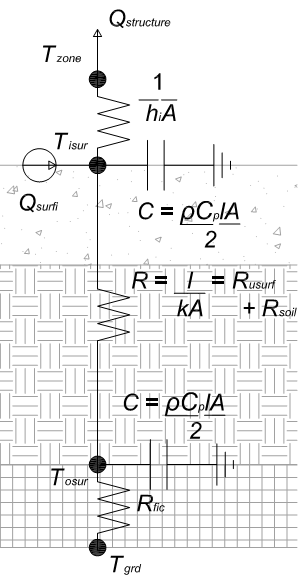
\includegraphics[scale=0.4]{jbs_figures/RC_2}
\caption{Modified RC network for underground surfaces}
\label{rc_underground}
\end{figure}

Using this method, one can use consistent equations for any wall type.  Since there is no air space adjacent to the exterior surface, there is no surface conductance ($h_{o}$). Instead, a fictitious insulating layer $R_{fic}$ is considered as the outer-most resistance for the BEM purpose.
The ground or the soil temperature is used as the ambient temperature $T_{amb}$ of underground walls.  The ground temperature is estimated using the mean air temperature and the location-specific published amplitude~\citep{american20152015}. Estimated average monthly ground temperatures at different geographic locations are available in the TMY dataset ~\citep{marion1995user}.  

Solar heat gain on opaque exterior surfaces $Q_{osurf}$ is calculated based on the buildings location and orientation in conjunction with the solar radiation intensity ~\citep{doe2016energyplus}:  

\begin{equation}
Q_{surfo} = \alpha(I_b\frac{S_s}{S}\cos\theta + I_sF_{ss} + I_gF_{sg})
\end{equation}

In essence, the solar heat gain is a relationship between the direct radiation, sky diffuse radiation, and ground reflected diffuse radiation, modified by various angle factors about the sun due to the orientation and geographic location of the surface. The intensities of radiation, $I_b$, $I_s$, and $I_g$ (beam, sky, and ground) are not measured directly but can be calculated from measured radiation (direct normal and diffuse horizontal) using the luminous efficacy models ~\citep{perez1990modeling}.  The Perez model is the basis of many modern solar models, including the approximate values given in the TMY dataset~\citep{marion1995user}. %Other approximations have been proposed by Muneer and Gueymard ~\citep{muneer2007solar,gueymard2009direct}.
Since, the real-time solar data is not available, the calculated input values for the surface solar heat gain is not dependent on actual weather conditions. Thus, for simplicity, the solar load values previously calculated by eQUEST is used as given in the current data. Since, only exterior surfaces are subject to direct solar radiation, they are assumed to have outer solar heat gain.

The the solar effect $U_o^j$ due to glazing is calculated using the solar heat gain coefficient (SHGC). The SHGC of the window represents the portion of solar radiation transmitted directly through the window, as well as the absorbed solar radiation, which is typically provided by the window manufacturer or can be assumed to be based on the window properties~\citep{american20132013}. Once the total solar radiation entering through the glazing is calculated, the solar flux on the interior walls $T_q$ can be estimated from it. There are several methods of calculating the solar heat flux on each interior surface $j$. In one such approach, it is assumed that all radiation first hits the floor of the space, and is reflected evenly across all the surfaces~\citep{o2010model}.

\begin{equation}
Q^k_{isol} = (1-\epsilon_{floor})H_{tot}\frac{\epsilon_k+\tau_k}{\sum\limits_{m=1}^{Nsurf}A_m(\epsilon_m+\tau_m)}
\end{equation}

In the current work, this internal solar gain $T_q$ is estimated as a part of the UQ framework.

Internal loads $Q_{int}$ are also unknown and is estimated through the WCSs-based UQ framework. Estimates of load schedules is based upon the BEM assumptions used by He at al.~\citep{he2016simplified}.  It is unlikely, however, that any physical building would follow the exact prescribed schedules with precision. Thus an optimal estimation method becomes necessary, especially due to the involved high-dimensional system.

%The airflow due to infiltration is another unknown and has been included in the internal load estimation.  
The infiltration rate at any given time is based upon the pressure differential between the building and the exterior environment, as well as the effective leakage area of the building.  The expected pressure difference across each leak is calculated as follows ~\citep{american20132013}:

\begin{equation}
\Delta p=0.0129s^2C_pP_U+HP_T+\Delta p_I
\end{equation}

The pressure difference is a combination of the shelter factor $s$, the estimated wind pressure coefficient $C_p$, the reference wind parameter $P_U$, the height of the building $H$, stack effect parameter $P_T$, and the building mechanical pressure differential $\Delta p_I$.  These parameters depend on air temperature, air density, wind speed, and wind direction, and the resulting differential is modified by the nature of the building openings.  To obtain an accurate, effective leakage area, a blower door test is required, pressurizing the space to a specified value ~\cite{american20132013}. For a large building, this is a costly process.  Consequently, the estimated peak infiltration rate is simply based on an assumed construction tightness.  
%Because of the involved uncertainty, the infiltration rate is also estimated with the other internal loads.

Most thermal zones also have furniture in the space that provides thermal mass and additional surfaces for radiation.  Specific information on the furniture in the zone, especially thermal properties, is difficult to obtain.  Wang and Xu~\citep{wang2006parameter} use a 2C2R model to estimate the internal mass of a zone using a genetic algorithm; however, the resulting parameters have no physical meaning other than an assumed lumped mass for estimation purposes.  Therefore, the state space equations in this work do not directly include any effects due to internal mass. Internal mass effects are included in the internal load estimation. 

In the presented case study, there are zone-level HVAC units such as hot water baseboard radiation. These baseboard units provide conditioning to the zone.  The Building Management System (BMS) controls and monitors these baseboard units that work in conjunction with the supply air flows and temperatures.  The baseboard units are included as a special case of the internal load. Like the HVAC parameters, the eQUEST hourly heat output values for the baseboard has been used.  In the case study, the BMS tracks the operation of the control valve, which can be used with the design flow rates and actual hot water loop temperatures to approximate the unit heat output.  This value is then simply subtracted from the calculated internal load.  

\subsection{Identification of Weakly Connected Subsystems and Optimal Estimation}
\label{WCS}

Optimal estimation of the unknown variables $T_i,T_o, T^{int}$ and $T_q$ in the problem detailed in Section~\ref{problem} refers to solving the following minimization problem
\begin{equation}
\displaystyle \min_{\hat{\textbf{x}}_k} E\left[|| \textbf{x}_k - \hat{\textbf{x}}_k ||_2 \right]
\end{equation}
\noindent The above term refers to the error in the \textit{a posteriori} state estimation. For a given measurement $\textbf{z}_t$, solution to the problem is same as solving the well known \textit{Filtering} problem. Consider the solution at time $t-1$ as $\hat{\textbf{x}}_{t-1}$ and covariance $\Sigma_{t-1}$, the estimate $\hat{\textbf{x}}_t$ and covariance $\Sigma_t$ are given as,

\begin{equation}
\label{kalman_full}
\begin{array}{l}
\hat{\textbf{x}}_t = \hat{\textbf{x}}_{t|t-1} + K\textbf{y}_{t} \\
\Sigma_t = \Sigma_{t|t-1} - K (R + C \Sigma_{t|t-1} C^T)  K^T
\end{array}
\end{equation}

\noindent where $K$ is known as the Kalman gain and $\textbf{y}_t = \textbf{z}_t - \hat{\textbf{x}}_{t|t-1}$ is known as the measurement residual. The \textit{a priori} estimates $\hat{\textbf{x}}_{t|t-1}$ and $\Sigma_{t|t-1}$ are one step solution to the Equation~\ref{state_space} depending on $\hat{\textbf{x}}_{t-1}$ and covariance $\Sigma_{t-1}$. The expression for the Kalman gain $K$ is given as~\citep{kalman1960new},

\begin{equation}
K = \Sigma_{t|t-1} C \left( R + C \Sigma_{t|t-1} C^T \right) ^{-1}
\end{equation}

Due to the high dimensionality of the problem involving large number of state variables $N$, the series of matrix operations becomes computationally expensive. To increase computational efficiency, the above filtering problem is solved through Identification of Weakly Connected Subsystems (WCSs)~\citep{Mukherjee_2017,mukherjee2015laplacian,mukherjee2015non}. The WCS-based method is effective in solving high-dimensional UQ problems involving linear and non-linear filtering problems. %The figure illustrates how the state variable $\mathbf x \in \mathbb{R} ^n$ is decomposed into WCSs. 

WCSs for the state variable $\textbf{x} \in \mathbb{R}^N$ are the countable, mutually exclusive and exhaustive partitions $\textbf{y}_j  \in \mathbb{R}^{n_j}$, such that the following relation holds 
\begin{equation}
\begin{array}{l}
\displaystyle P(\textbf{x}_t) = \prod_j P(\textbf{y}_{j_t}) \\ 
\sum_j n_j = N
\end{array}
\end{equation}

The index $t$ represents that the relation is invariant under the transformation given by Equation~\ref{state_space} for a time-period $t \in [0, T)$. Performing such decomposition of $\textbf{x}_t$ enables faster UQ by solving parallel subproblems known given as:

\begin{equation}
\label{sub-problem}
\dot{\textbf{y}}_{j} = A_j(t)\textbf{y}_{j} + B_j \textbf{u}_j
\end{equation}

The solutions to each subproblem in Equation~\ref{sub-problem} is given by the following continuous time Kalman filter~\citep{jazwinski2007stochastic}:

\begin{equation}
\begin{array}{l}
\displaystyle \dot{E(\textbf{y}_{j})} = A_j(t)E(\textbf{y}_{j}) + B_j \textbf{u}_j + K_j(z_j - C_j E(\textbf{y}_{j_t})) \\
\displaystyle \dot{\Sigma_j} = A_j(t)\Sigma_j + \Sigma_j A_j(t)^T - K_j R_j K_j^T \\
\displaystyle K_j = \Sigma_j A_j^T R_j^{-1}
\end{array}
\end{equation}

\noindent This invokes the use parallel computation for both the one-step \textit{a priori} estimation and as well the use of Kalman filter for the \textit{a posteriori} estimation. The state estimates $\textbf{x}_t$ and $\Sigma_t$ are computed from the WCSs using \textit{direct sum} of the vector spaces as,

\begin{equation}
\label{jbs:moment_cl}
\begin{array}{l}
E(\textbf{x}_t) = E(\textbf{y}_{1_t}) \oplus E(\textbf{y}_{2_t}) \oplus \ldots \oplus E(\textbf{y}_{m_t}) \\
\Sigma_t = \displaystyle \bigoplus_j \Sigma_{j_t} = \text{diag}\left( \Sigma_{1_t}, \ldots, \Sigma_{m_t}  \right)
\end{array}
\end{equation}

The normalized symmetrized adjacency matrix derived from the state-space matrix $A = \left( a_{ij}  \right)$ in Equation~\ref{state_space}~\citep{Mukherjee_2017} is given as:

\begin{equation}
\label{symm}
W = 0.5 (D^{-1} A_{abs} + A_{abs}^T D^{-1})
\end{equation}

\noindent where, $A_{abs} = \left( | a_{ij} | \right)$ and $D$ is the corresponding degree matrix of $A_{abs}$. The clusters are identified using Louvain method of community detection~\citep{blondel2008fast}. The method identifies weakly connected components in a weighted graph by maximizing modularity function defined as:

\begin{equation}
Q = \frac{1}{2m_q} \displaystyle \sum_{i,j} \left[W_{i,j} - \frac{k_i k_j}{2m_q} \right] \delta(c_i, c_j)
\end{equation}

\noindent where, $m_q = \sum_{i,j}W_{i,j} = N/2$, $k_i = \sum_i W_{i,j}$ and $c_i$ is the partition to which $i^{\text{th}}$ state belongs. The delta function $\delta(c_i,c_j)$ is 
\begin{equation}
\delta(c_i,c_j) = \begin{cases}
1 & c_i = c_j \\ 0 & \text{otherwise}
\end{cases}
\end{equation}
Maximizing $Q$ gives the values of $c_i$'s, $i = 1$ to $N$ and hence determines the cluster structure. In the next section, details pertaining to a building used for BEM modeling purposes is outlined.




\section{BEM Details}
\label{case_study}

The case study building used in this work to illustrate the efficiency of the outlined UQ framework is a College/University building in Central New York, United States(see Figure~\ref{building}). The facility is an existing 4-story 54,362 square feet building with a mechanical penthouse.  It is comprised of primarily classrooms and offices, student lounges, conference rooms, observation rooms and as well as other support spaces.  The lowest floor comprises of underground zones and the northeast portion of the building is attached to an adjacent structure.

\begin{figure}[H]
\centering
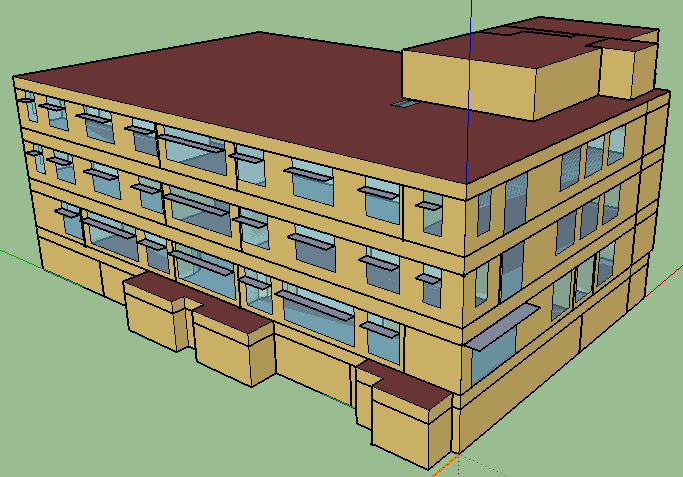
\includegraphics[scale=0.4]{jbs_figures/building}
\caption{Schematic of College/University building in Central New York used for creating the case study BEM}
\label{building}
\end{figure}

The individual spaces are conditioned at the zone level by fan-coil units with fin-tube radiation in the perimeter spaces.  A dedicated outdoor air system supplies tempered ventilation air directly to the fan-coil units.  The hot- and chilled-water coils are supplied from the campus plants.  Network data rooms are conditioned separately with a variable refrigerant flow heat pump system.  The brick and Concrete Masonry Unit(CMU) envelope has a combination of rigid and spray-applied insulation at the exterior walls, and the high-albedo Ethylene Propylene Diene-Terpolymer membrane(EPDM) roof is concrete deck topped with rigid insulation. The windows are tinted high-performance glazing with sunshades on the southern fenestration. The building uses high-efficiency LED lighting with occupancy sensors and daylighting controls. The building operates Monday through Friday from 7 am to 10 pm.

Thermal Zones are determined by the actual HVAC design that breaks up the building by space use and orientation.  There are a total of 132 zones in the building, including unconditioned plenum spaces above the ceilings, for 61 directly conditioned zones.  In the modeled building, there are 668 interior surfaces, 69 underground surfaces (including slab-on-grade floors), 124 exterior surfaces (including roofs), and 80 windows.  The second-floor thermal zones are shown in Figure~\ref{floor_plan}.

\begin{figure}[H]
\centering
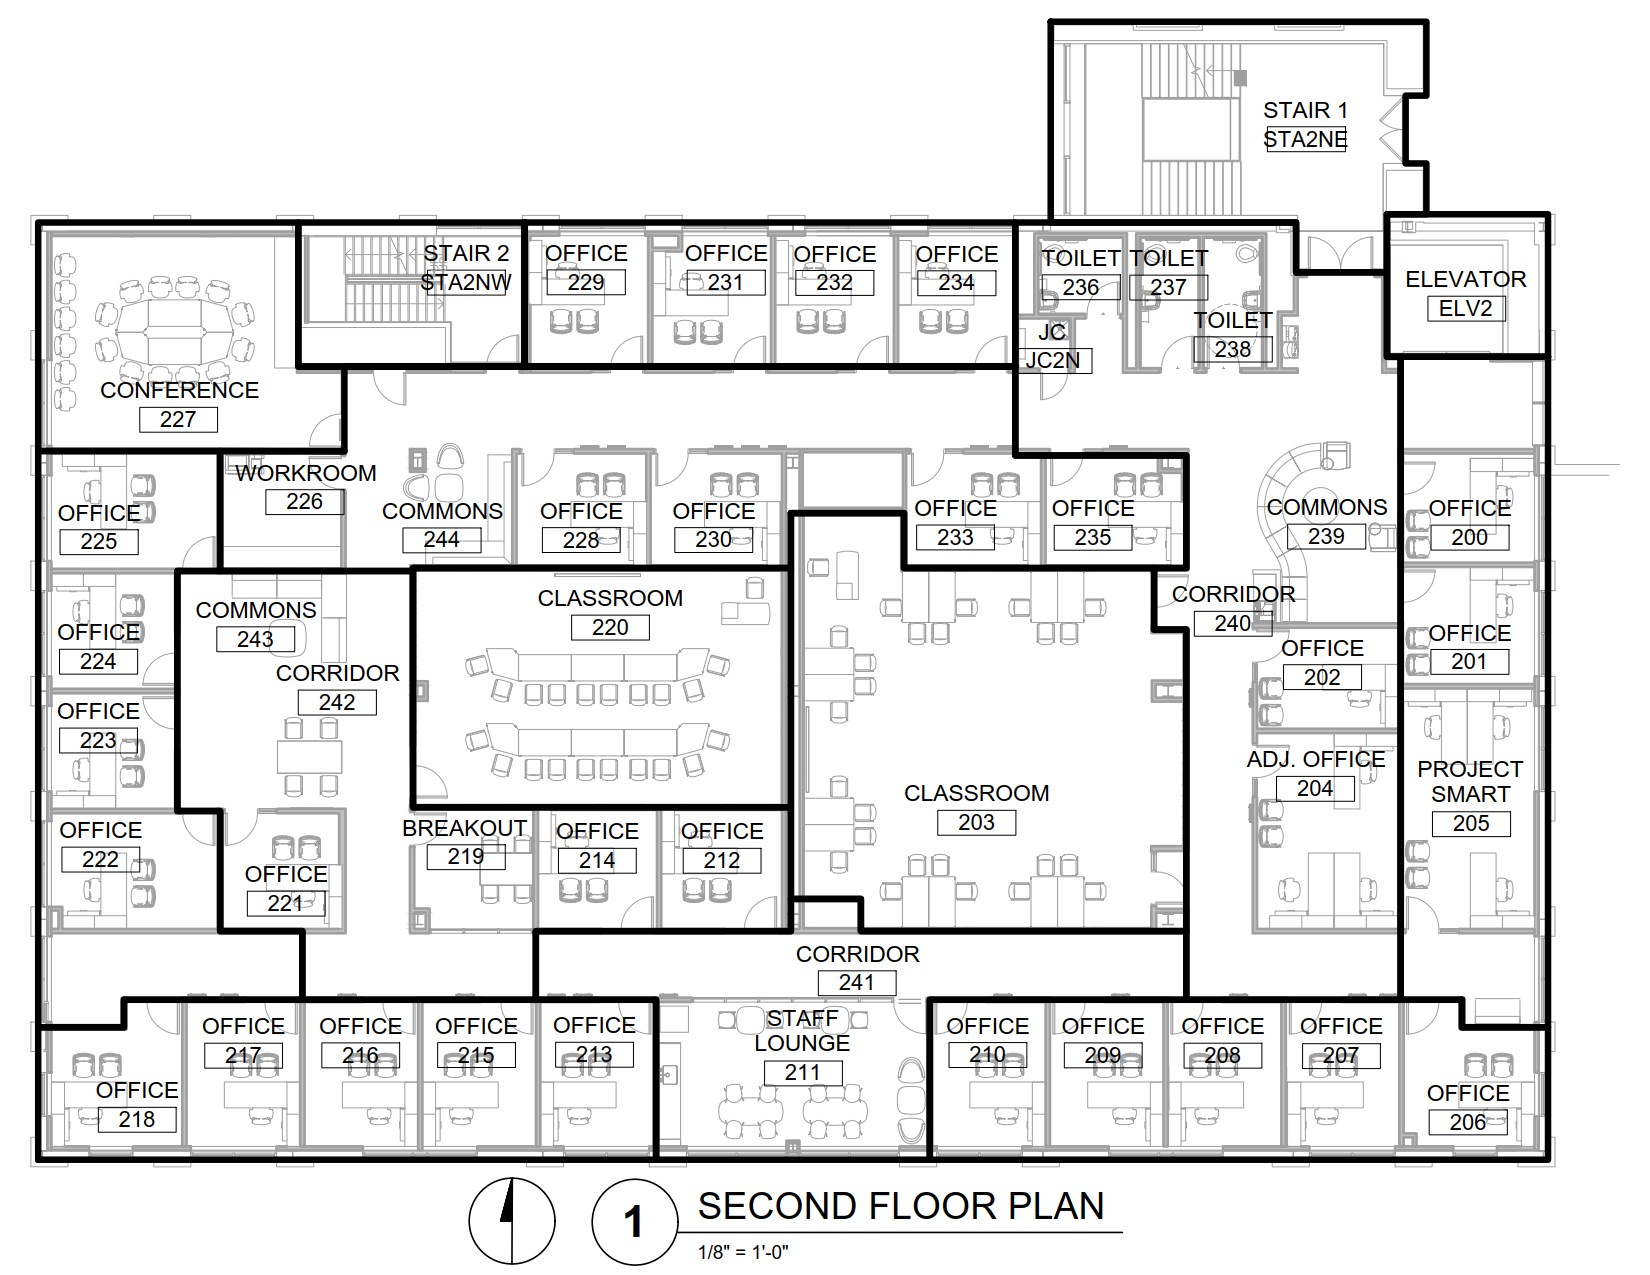
\includegraphics[scale=0.4]{jbs_figures/floor_plan}
\caption{Second Floor Thermal Zones of the BEM}
\label{floor_plan}
\end{figure}

Four zones are specifically considered to illustrate the details of our methodology. These are a ground floor perimeter zone with underground walls (Zone 1), a first floor exterior zone with west facing windows (Zone 47), a second floor zone with no exterior surfaces (Zone 80), and a third floor zone with a roof and south and east exterior walls (Zone 97).  The number of input parameters needed per zone to calculate only conduction through building surfaces is listed in Table~\ref{zonetable}.  Each zone also has dynamic input parameters for lighting, occupancy, equipment load, and infiltration, as well as numerous inputs to simulate the HVAC system and assumptions by the BEM program.  Each of these inputs has uncertainty associated with them. As these zones represent only 4 out of the 132 zones, it is clear that this is a high-dimensional problem that requires a scalable UQ method. 

\begin{table}[H]
\begin{center}
\caption{BEM Inputs per Zone - Conduction through Surfaces Only}
\resizebox{\textwidth}{!}{ 
\begin{tabular}{cccccccc}
\hline
& Number of & Number of & Number of & & Number of  & Number of & Number of \\ 
& Exterior & Interior & Underground & Number of & Construction & Adjacent & BEM Input \\ 
& Surfaces & Surfaces & Surfaces & Windows & Materials & Zones & Parameters\\ 
\hline
Zone 1 & 0 & 6 & 4 & 0 & 11 & 2 & 52 \\
Zone 47 & 2 & 12 & 0 & 2 & 11 & 3 & 80 \\
Zone 80 & 0 & 6 & 0 & 0 & 10 & 4 & 48 \\
Zone 97 & 2 & 8 & 0 & 6 & 14 & 4 & 81 \\
\hline
\end{tabular}
}
\label{zonetable}
\end{center}
\end{table}

This building has been modeled in eQUEST (version 3.65)~\citep{hirsch2006equest} following the methodology laid out in ASHRAE 90.1-2013 (Appendix G ~\citep{american90}).  All known parameters of the building, as discussed in Section~\ref{case_study}, have been input into the software program. eQUEST uses the heat-balance method in a forward approach. At first it calculates the space load at each time step. This is followed by converting the space load into the required load and conditions of the HVAC system. The calculated load is fed back into the load calculation~\citep{hirsch2003doe}.  The process for calculating building energy use is depicted in Figure~\ref{process}. For the outdoor conditions present at the building site, Typical Meteorological Year (TMY) dataset is used for the nearest city, Syracuse NY~\citep{marion1995user}. The TMY data is not representative of any particular year but is developed to represent the typical conditions of a given location.

\begin{figure}[H]
\centering
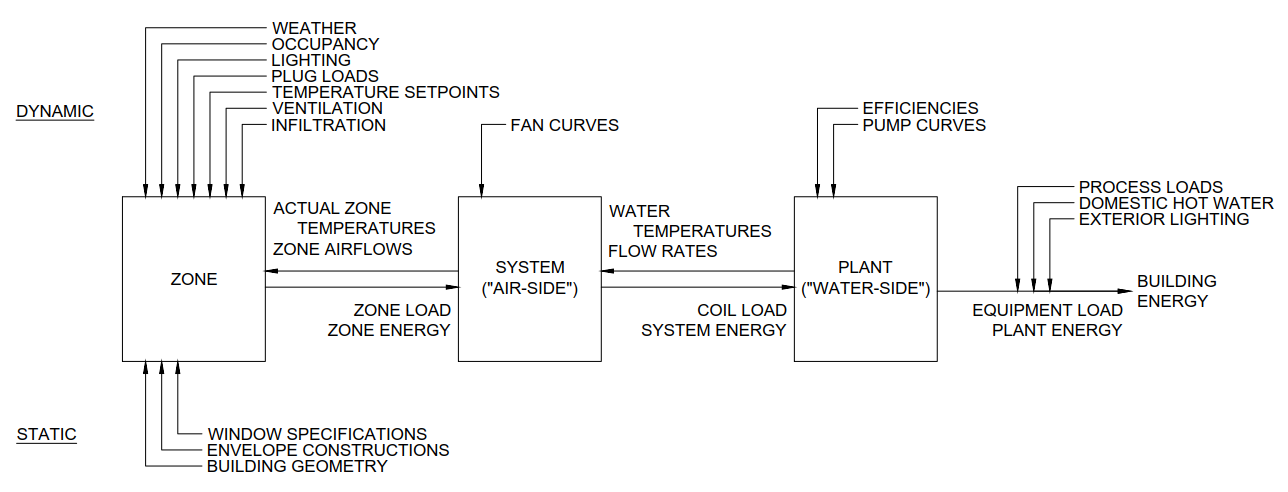
\includegraphics[scale=0.45]{jbs_figures/process}
\caption{Schematic for calculation of building energy}
\label{process}
\end{figure}

Since the modeled building has a digital building management system, one has access to the HVAC airflows and temperatures, water flow rates and temperatures, zone temperatures, as well as a variety of other control points and HVAC system. \textcolor{red}{However, eQUEST outputs which are data points known to be tracked by the building management system, including zone temperatures, are taken as a given in our state equation; the control points for the fan-coil units are shown in Table~\ref{controls}.  Thus the eQUEST results are used as the actual observed results.}  Calculating the HVAC system inputs for the heat balance equation requires specific information on fan curves, coil properties, pump curves, pressure losses, control strategies, capacity curves, etc. All of these is provided to the model. Furthermore, there is a feedback loop relationship between the HVAC output and the building load components~\citep{he2016simplified}. Because of the complexity in calculating the air-side HVAC parameters and because the data required for this analysis are typically readily available with a robust building controls system, the hourly air temperatures and flows calculated by eQUEST are used in our state equations.  

\begin{table}[H]
\begin{center}
\caption{Fan Coil Unit Control Points\\}
\small
\begin{tabular}{|l|c|c|c|c|}
\hline
& Analog & Analog & Digital & Digital \\ 
Description & Input & Output & Input & Output\\ 
\hline \hline
Fan Enable/Disable & & & & X\\
\hline
Fan Status & & & X & \\
\hline
Space Temperature & X & & &\\
\hline
Heating Valve Position & & X & & \\
\hline
Cooling Valve Position & & X & & \\
\hline
Leaving Air Temperature & X & & & \\
\hline
Filter Pressure Differential Sensor & & & X & \\
\hline
Condensate Alarm & & & X & \\
\hline
\end{tabular}
\label{controls}
\end{center}
\end{table}

In the eQUEST model, internal loads are assumed using hourly schedules. Lighting peak loads is calculated directly from the known lighting layout. However, the occupancy and receptacle loads are estimated.  Building code provides an approximation for the maximum occupancy for each space type~\citep{council2015international}, which provides an approximation.  Receptacle loads can be highly variable, especially with today’s proliferation of electronics. Typical representable load values have been compiled in COMNET~\citep{resnet2010}.  These peak load conditions are then scaled hourly based on estimated schedules.  The ASHRAE 90.1 User’s Manual provides typical fractional schedules for occupancy, zone lighting, and receptacle loads~\citep{americanenergy} that have been modified in this work. The building lighting in the modeled building is assumed to be  controlled by a combination of daylight harvesting controls, occupancy sensors, dimming switches, and manual on/off controls.  Using simple reduction factors, ASHRAE 90.1 provides guidance on the expected effect of some of the lighting controls ~\citep{american90}.  However, outcomes are not representative of a particular building, and it is likely that in practice, the actual hourly lighting power density would be substantially different than the predicted. 

The main floors of the modeled building is assumed to be partially attached to an adjacent building.  However, the adjacent building is controlled independently of the modeled building, and the properties of the adjacent building are assumed to be unknown. Therefore, the surface boundary conditions with the adjacent building are assumed to be adiabatic, with no heat transfer of any kind between the two buildings.  

The modeled building is used to demonstrate our proposed methodology largely due to its size and complexity.  With 61 directly conditioned thermal zones, one can explore the differences between and interconnectivity of perimeter zones and core zones.  There are several exterior wall construction types, as the first floor differs from the upper floors, and the underground walls require a modified approach to calculate the heat transfer.  Lighting controls, including photo-sensors, create a further challenge for the internal load estimation.  There are a vast number of input parameters, that necessitates the use of a scalable UQ method that can tackle scalable high-dimensional problems.

%There is extensive documentation for the building, as the design for a major building renovation was recently completed, including construction drawings and specifications.  Since this is an actual building, where physical limitations and unknown constraints may have dictated the design.  Although there is no access to the data from the building control system which shows the real-time building temperatures and HVAC use, the control points and sequence of operation are accessible, which dictate what information is recorded by the building management system.  


\section{Results}
\label{results}
\subsection{Adjacency and Cluster Analysis}
\label{adjacency}

The BEM described in Section~\ref{case_study} contains 2649 state variables (Involving $\lbrace T_k,T_o,T_i,T_q,T^{int} \rbrace$), with 1125 input variables. The state-space equation (in Equation~\ref{state_space}) of the BEM is based on the thermal properties of the materials of the building and the interaction of the zonal and wall temperatures. The adjacency matrix $W$ is a reflection of coupling along with the presence of any inter-zone coupling. The variable $T_{out}^j$ in Equation~\ref{zone_equation} can be both the ambient temperature $T_{amb}$ or the temperature of adjacent zone. Thus, the inter-zone coupling (if present) depends on the magnitude of $h^j_o A_j/C_j$. Additionally, the adjacency matrix is highly sparse. This makes a visual representation of the whole $W$ very difficult to interpret. Results assimilated from the four thermal zones listed in Table~\ref{zonetable} representing diverse zonal conditions: Zone 1, Zone 47, Zone 80 and Zone 97 are discussed next.   

\begin{figure}[H]
\begin{subfigure}{0.45\textwidth}
\centering
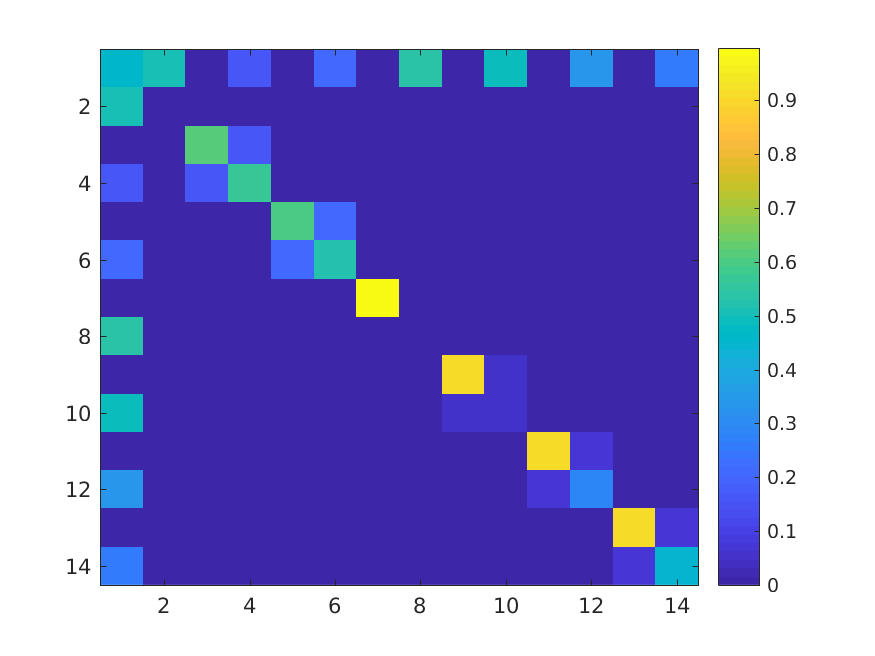
\includegraphics[width=\textwidth]{jbs_figures/adj_1}
\caption{}
\label{adj_1}
\end{subfigure}
\centering
\begin{subfigure}{0.45\textwidth}
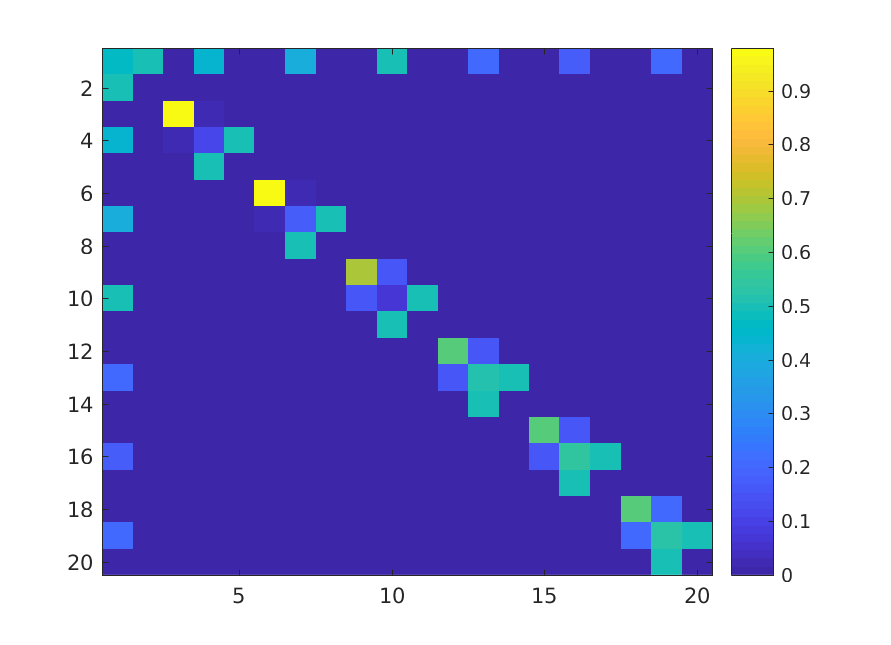
\includegraphics[width=\textwidth]{jbs_figures/adj_2}
\caption{}
\label{adj_2}
\end{subfigure} \\
\begin{subfigure}{0.45\textwidth}
\centering
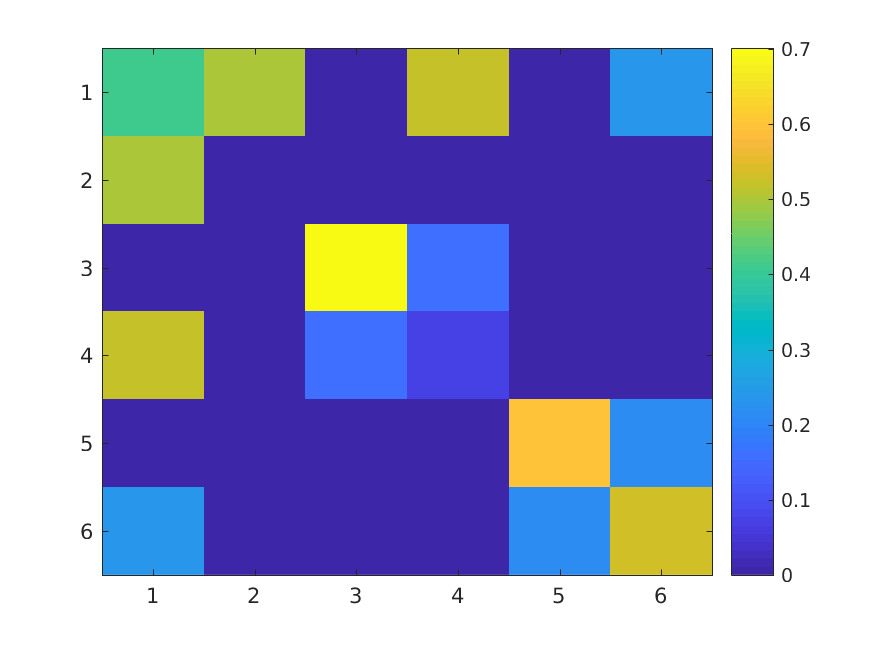
\includegraphics[width=\textwidth]{jbs_figures/adj_3}
\caption{}
\label{adj_3}
\end{subfigure}
\centering
\begin{subfigure}{0.45\textwidth}
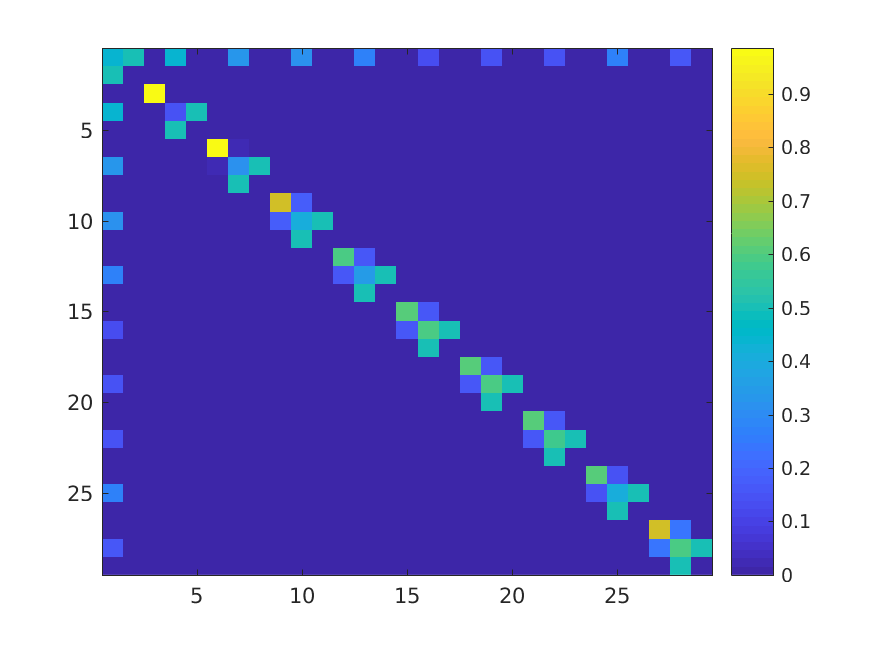
\includegraphics[width=\textwidth]{jbs_figures/adj_4}
\caption{}
\label{adj_4}
\end{subfigure}
\caption{Normalized Adjacency Information for (a) Zone 1, (b) Zone 47, (c) Zone 80 and (d) Zone 97}
\label{fig:Zone_adjacency}
\end{figure}


Figure~\ref{fig:Zone_adjacency} shows the sub-matrices of the Normalized Adjacency matrix $W$ corresponding to the four zones. The zones show the involved variables $T_k,T_o,T_i,T^{int}$. Zone 1 and 80 do not belong to exterior zones (zones having window). Thus the variable $T_q$ is absent from the corresponding adjacency figures (Figures~\ref{fig:Zone_adjacency}(a) and (c)). To demonstrate the inter-zone coupling between these four zones Figure~\ref{adj_new} has been plotted. The plot shows no interaction between these four zones. However, this result does not conclude that there is zero interaction between other zones.

\begin{figure}[H]
\centering
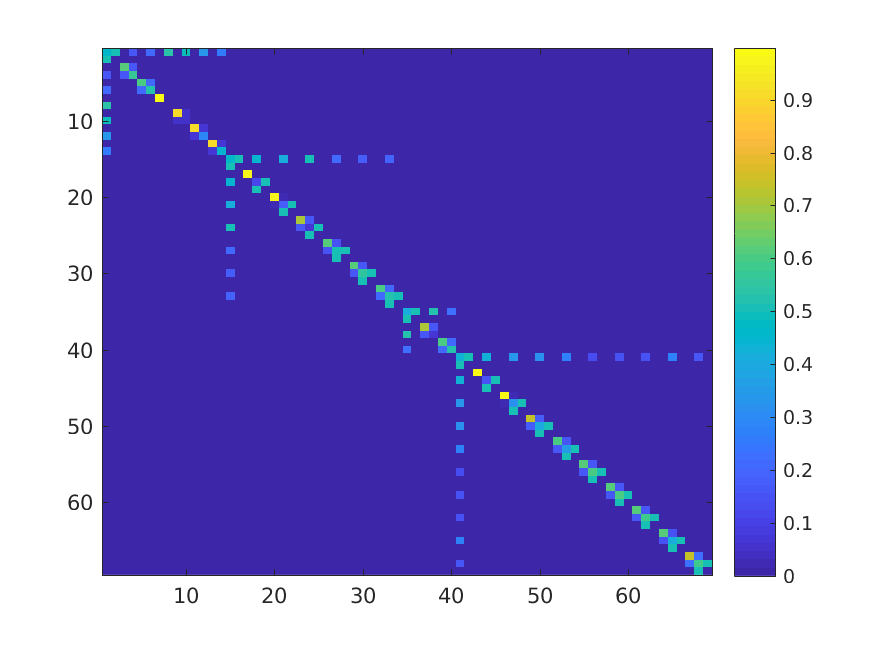
\includegraphics[width=0.8\textwidth]{jbs_figures/adj_comb}
\caption{Adjacency Matrix for Zone 1, Zone 47, Zone 80 and Zone 97 combined }
\label{adj_new}
\end{figure}

The cluster matrix is displayed in Figure~\ref{cluster_matrix}. 

\begin{figure}[H]
\centering
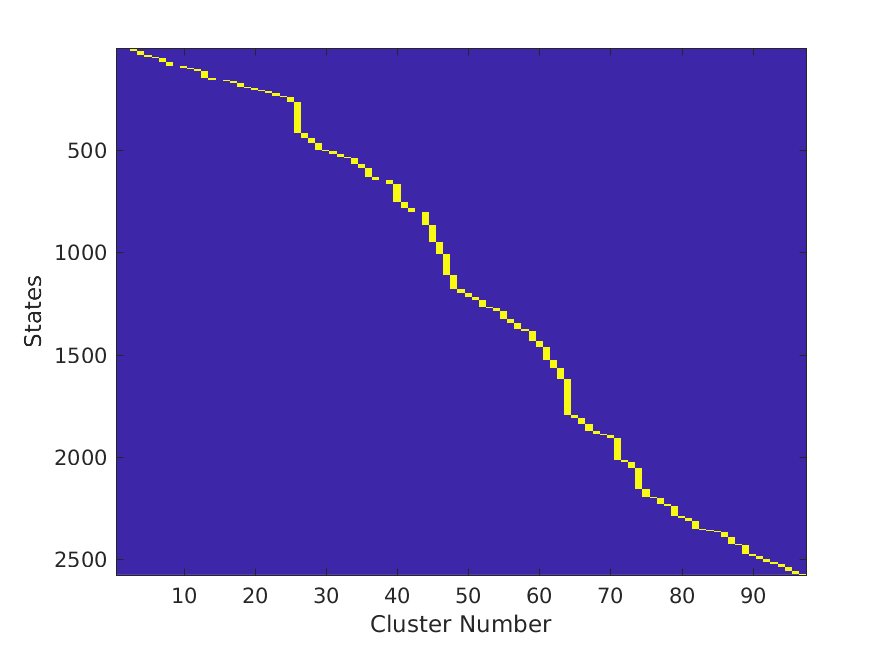
\includegraphics[width=0.8\textwidth]{jbs_figures/cluster_matrix}
\caption{Cluster Matrix}
\label{cluster_matrix}
\end{figure}

The application of the Louvain modularity optimization-based clustering algorithm on the derived $W$ matrix for 2649 states resulted in identification of $m=97$. The number of identified clusters ($m=97$) is less than the number of zones(=132). However, the cluster structure works in accordance with the adjacency information identified in Figure~\ref{fig:Zone_adjacency} and~\ref{adj_new}. It can be observed in Figure~\ref{cluster_matrix} that consecutive states participate in clusters. Intuitively in can be concluded that the clustering algorithm either recognizes a single zone or a group of zones as a cluster. In most cases it ignores the inter-zone coupling. In the next section, the whole system is analyzed along with the estimation of the thermal loads via these identified clusters or WCSs. To compare the performance of the WCS-based UQ, the whole BEM is also analyzed without any clustering.

\subsection{Estimated Temperatures and Thermal Loads}

For the simulation, a measurement noise is assumed for each of the zonal temperature as $R = \text{diag}\lbrace r_1, r_2, \ldots, r_{132} \rbrace$ where $\lbrace r_1, r_2, \ldots, r_{132} \rbrace$ are randomly generated numbers between 0 and $0.5$. This corresponds to the accuracy of typical room temperature sensor~\citep{siemens2013catalog}. 
Before displaying the estimated thermal loads, the accuracy of the WCS-based UQ algorithm is demonstrated first by a plot of error in estimation metric vs time similar to our previous works~\ref{chap:wcs}. This metric is computed at each time as:

\begin{equation}
\label{jbs:err_metric}
e_{\mu} = \begin{Vmatrix}
\frac{E(\textbf{x}_{t_c}) - E(\textbf{x}_{t_f})}{E(\textbf{x}_{t_f})}
\end{Vmatrix}_2
\end{equation}

\noindent where, $E(\textbf{x}_{t_c})$ is the mean of the state variable $\textbf{x}_t \in \mathbb{R}^n$ obtained from the Equation~\ref{jbs:moment_cl}. $E(\textbf{x}_{t_f})$ is obtained by running the full model (Equation~\ref{kalman_full}). Figure~\ref{jbs:fig:error} shows the plot of $e_{\mu}$ vs time for a span of one year.  


\begin{figure}[H]
\centering
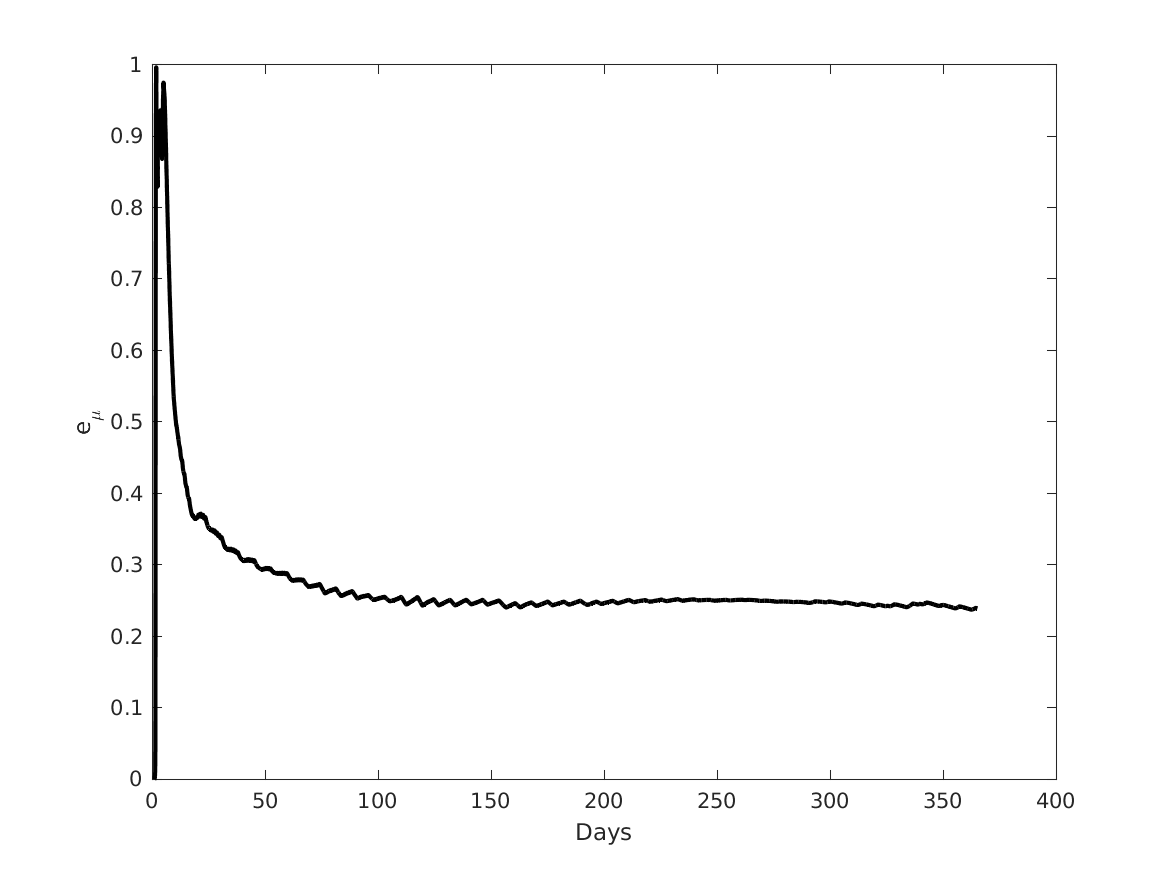
\includegraphics[width=\textwidth]{jbs_figures/fig2}
\caption{Plot of error in estimation vs time}
\label{jbs:fig:error}
\end{figure}

The plot shows the accuracy of the WCS-based UQ approach. It has already been established to work very good for a linear system~\citep{Mukherjee_2017}. The identified WCSs ignore the inter-zone mixing of the wall temperatures. This mixing shows to have very little effect on the results. The error metric $e_{\mu}$ rises to 1 in the initial days and converges to a value between 0.2 and 0.3 (20-30$\%$) towards the later part of the year. The slow convergence is might be due to large number of state variables compared to fewer observations. Also, the individual zonal temperatures are not an explicit function of the surface temperatures. This causes difficulty in the estimation of the surface temperatures $T_o$ and $T_i$ from $T_k$. Due to this convergence rate, subsequent analysis has been shown skipping the first month of the year. 
Figure~\ref{fig:Zone_temperature} shows the accuracy in estimating the zonal temperatures for the four zones; Zone 1, Zone 47, Zone 80, and Zone 97. The observed values for each plot is shown to lie between the $\mu \pm 3 \sigma$ limits for each zonal temperature $T_k$. 


\begin{figure}[H]
\begin{subfigure}{0.45\textwidth}
\centering
\includegraphics[width=\textwidth]{jbs_figures/zone_1}
\caption{}
\label{zone_1}
\end{subfigure}
\centering
\begin{subfigure}{0.45\textwidth}
\includegraphics[width=\textwidth]{jbs_figures/zone_2}
\caption{}
\label{zone_2}
\end{subfigure} \\
\begin{subfigure}{0.45\textwidth}
\centering
\includegraphics[width=\textwidth]{jbs_figures/zone_3}
\caption{}
\label{zone_3}
\end{subfigure}
\centering
\begin{subfigure}{0.45\textwidth}
\includegraphics[width=\textwidth]{jbs_figures/zone_4}
\caption{}
\label{zone_4}
\end{subfigure}
\caption{Estimated Temperature for (a) Zone 1, (b) Zone 47, (c) Zone 80 and (d) Zone 97}
\label{fig:Zone_temperature}
\end{figure}

% \begin{figure}[H]
% \centering
% \subfigure[Zone 1]{\includegraphics[width=0.45\textwidth]{figures/zone_1}}
% \subfigure[Zone 33]{\includegraphics[width=0.45\textwidth]{figures/zone_2}} \\
% \subfigure[Zone 80]{\includegraphics[width=0.45\textwidth]{figures/zone_3}}
% \subfigure[Zone 97]{\includegraphics[width=0.45\textwidth]{figures/zone_4}}
% \caption{Adjacency Information for (a) Zone 1, (b) Zone 47, (c) Zone 80 and (d) Zone 97}
% \label{Zone_temperature}
% \end{figure}



Figures~\ref{fig:Zone_Int_temperature_feb},~\ref{fig:Zone_Int_temperature_june}~\ref{fig:Zone_Int_temperature_oct} show the estimated internal loads for the four specific zones for the month of February, June and October respectively. The internal loads loosely track occupancy, as expected, and have daily peaks midday and drop at night.  The internal load values typically increase daily during weekdays, before decreasing over the weekends.  This is likely due to the high thermal mass associated with the space, particularly the floor and the exterior walls, which allows the space to retain heat at night, and provides an increased baseline internal load each day.  Zone 1, for example, has an especially high thermal capacitance due to the surrounding soil, which minimizes the temperature drop in the evenings.         

Because the model has approximately 2700 state variables, and only 132 outputs, the resulting estimations are equally distributed based on the coefficients of the state space coefficients, and the estimated results follow a pattern similar to the estimated zonal temperatures.  The assumption that the internal loads are slow-changing with a $\dot{T}_k^{int} = 0$ minimizes the estimated nightly reduction in internal load, since it does not permit a drastic change.  Note that these values include the uncertainty due to the baseboard heat.     


% \begin{figure}[H]
% \centering
% \subfigure[Zone 1]{\includegraphics[width=0.45\textwidth]{figures/load_1_2}}
% \subfigure[Zone 33]{\includegraphics[width=0.45\textwidth]{figures/load_2_2}} \\
% \subfigure[Zone 80]{\includegraphics[width=0.45\textwidth]{figures/load_3_2}}
% \subfigure[Zone 97]{\includegraphics[width=0.45\textwidth]{figures/load_4_2}}
% \caption{Adjacency Information for (a) Zone 1, (b) Zone 33, (c) Zone 80 and (d) Zone 97 for the month of February}
% \label{Zone_Int_temperature_feb}
% \end{figure}

\begin{figure}[H]
\begin{subfigure}{0.45\textwidth}
\centering
\includegraphics[width=\textwidth]{jbs_figures/load_1_2}
\caption{}
\label{load_1_2}
\end{subfigure}
\centering
\begin{subfigure}{0.45\textwidth}
\includegraphics[width=\textwidth]{jbs_figures/load_2_2}
\caption{}
\label{load_2_2}
\end{subfigure} \\
\begin{subfigure}{0.45\textwidth}
\centering
\includegraphics[width=\textwidth]{jbs_figures/load_3_2}
\caption{}
\label{load_3_2}
\end{subfigure}
\centering
\begin{subfigure}{0.45\textwidth}
\includegraphics[width=\textwidth]{jbs_figures/load_4_2}
\caption{}
\label{load_4_2}
\end{subfigure}
\caption{Estimated Internal Thermal Load for (a) Zone 1, (b) Zone 47, (c) Zone 80 and (d) Zone 97 for the month of February}
\label{fig:Zone_Int_temperature_feb}
\end{figure}

% \begin{figure}[H]
% \centering
% \subfigure[Zone 1]{\includegraphics[width=0.45\textwidth]{figures/load_1_6}}
% \subfigure[Zone 33]{\includegraphics[width=0.45\textwidth]{figures/load_2_6}} \\
% \subfigure[Zone 80]{\includegraphics[width=0.45\textwidth]{figures/load_3_6}}
% \subfigure[Zone 97]{\includegraphics[width=0.45\textwidth]{figures/load_4_6}}
% \caption{Adjacency Information for (a) Zone 1, (b) Zone 33, (c) Zone 80 and (d) Zone 97 for the month of June}
% \label{Zone_Int_temperature_june}
% \end{figure}

\begin{figure}[H]
\begin{subfigure}{0.45\textwidth}
\centering
\includegraphics[width=\textwidth]{jbs_figures/load_1_6}
\caption{}
\label{load_1_6}
\end{subfigure}
\centering
\begin{subfigure}{0.45\textwidth}
\includegraphics[width=\textwidth]{jbs_figures/load_2_6}
\caption{}
\label{load_2_6}
\end{subfigure} \\
\begin{subfigure}{0.45\textwidth}
\centering
\includegraphics[width=\textwidth]{jbs_figures/load_3_6}
\caption{}
\label{load_3_6}
\end{subfigure}
\centering
\begin{subfigure}{0.45\textwidth}
\includegraphics[width=\textwidth]{jbs_figures/load_4_6}
\caption{}
\label{load_4_6}
\end{subfigure}
\caption{Estimated Internal Thermal Load for (a) Zone 1, (b) Zone 47, (c) Zone 80 and (d) Zone 97 for the month of June}
\label{fig:Zone_Int_temperature_june}
\end{figure}


% \begin{figure}[H]
% \centering
% \subfigure[Zone 1]{\includegraphics[width=0.45\textwidth]{figures/load_1_10}}
% \subfigure[Zone 33]{\includegraphics[width=0.45\textwidth]{figures/load_2_10}} \\
% \subfigure[Zone 80]{\includegraphics[width=0.45\textwidth]{figures/load_3_10}}
% \subfigure[Zone 97]{\includegraphics[width=0.45\textwidth]{figures/load_4_10}}
% \caption{Adjacency Information for (a) Zone 1, (b) Zone 33, (c) Zone 80 and (d) Zone 97 for the month of October}
% \label{Zone_Int_temperature_june}
% \end{figure}

\begin{figure}[H]
\begin{subfigure}{0.45\textwidth}
\centering
\includegraphics[width=\textwidth]{jbs_figures/load_1_10}
\caption{}
\label{load_1_10}
\end{subfigure}
\centering
\begin{subfigure}{0.45\textwidth}
\includegraphics[width=\textwidth]{jbs_figures/load_2_10}
\caption{}
\label{load_2_10}
\end{subfigure} \\
\begin{subfigure}{0.45\textwidth}
\centering
\includegraphics[width=\textwidth]{jbs_figures/load_3_10}
\caption{}
\label{load_3_10}
\end{subfigure}
\centering
\begin{subfigure}{0.45\textwidth}
\includegraphics[width=\textwidth]{jbs_figures/load_4_10}
\caption{}
\label{load_4_10}
\end{subfigure}
\caption{Estimated Internal Thermal Load for (a) Zone 1, (b) Zone 47, (c) Zone 80 and (d) Zone 97 for the month of October}
\label{fig:Zone_Int_temperature_oct}
\end{figure}

The solar gains for some of the walls for Zone 47 and Zone 97 are displayed in Figure~\ref{Zone_solar_temperature_feb}~\ref{Zone_solar_temperature_june}~\ref{Zone_solar_temperature_oct} for the three months. The graph shows an equal distribution of the solar load into the interior walls. This is an expected result, as eQuest models the radiation as uniformly distributed ~\citep{doe2016energyplus}; actual observed results would be likely to differ somewhat ~\citep{he2016simplified} due to the differences in direct and reflected solar radiation on the surfaces.  Note, too, that the surface heat flux somewhat tracks occupancy; this is likely due to the radiant heat output of the lighting in the space.  This is especially apparent at night, when the solar gain is expected to drop substantially, but some lighting remains on.  As with the internal loads, the solar gains follow a similar pattern to the estimated outputs due to the high number of estimated state variables. 

\begin{figure}[H]
\begin{subfigure}{0.45\textwidth}
\centering
\includegraphics[width=\textwidth]{jbs_figures/solar_2_2}
\caption{zone 47}
\label{solar_2_2}
\end{subfigure}
\centering
\begin{subfigure}{0.45\textwidth}
\includegraphics[width=\textwidth]{jbs_figures/solar_3_2}
\caption{Zone 97}
\label{solar_3_2}
\end{subfigure} 
\caption{Solar Gains for (a) Zone 47 and (b) Zone 97 for the month of February}
\label{Zone_solar_temperature_feb}
\end{figure}

% \begin{figure}[H]
% \centering
% \subfigure[Zone 1]{\includegraphics[width=0.45\textwidth]{figures/solar_2_2}}
% \subfigure[Zone 33]{\includegraphics[width=0.45\textwidth]{figures/solar_3_2}}
% \caption{Solar Gains for (a) Zone 47 and (b) Zone 97 for the month of February}
% \label{Zone_solar_temperature_feb}
% \end{figure}

\begin{figure}[H]
\begin{subfigure}{0.45\textwidth}
\centering
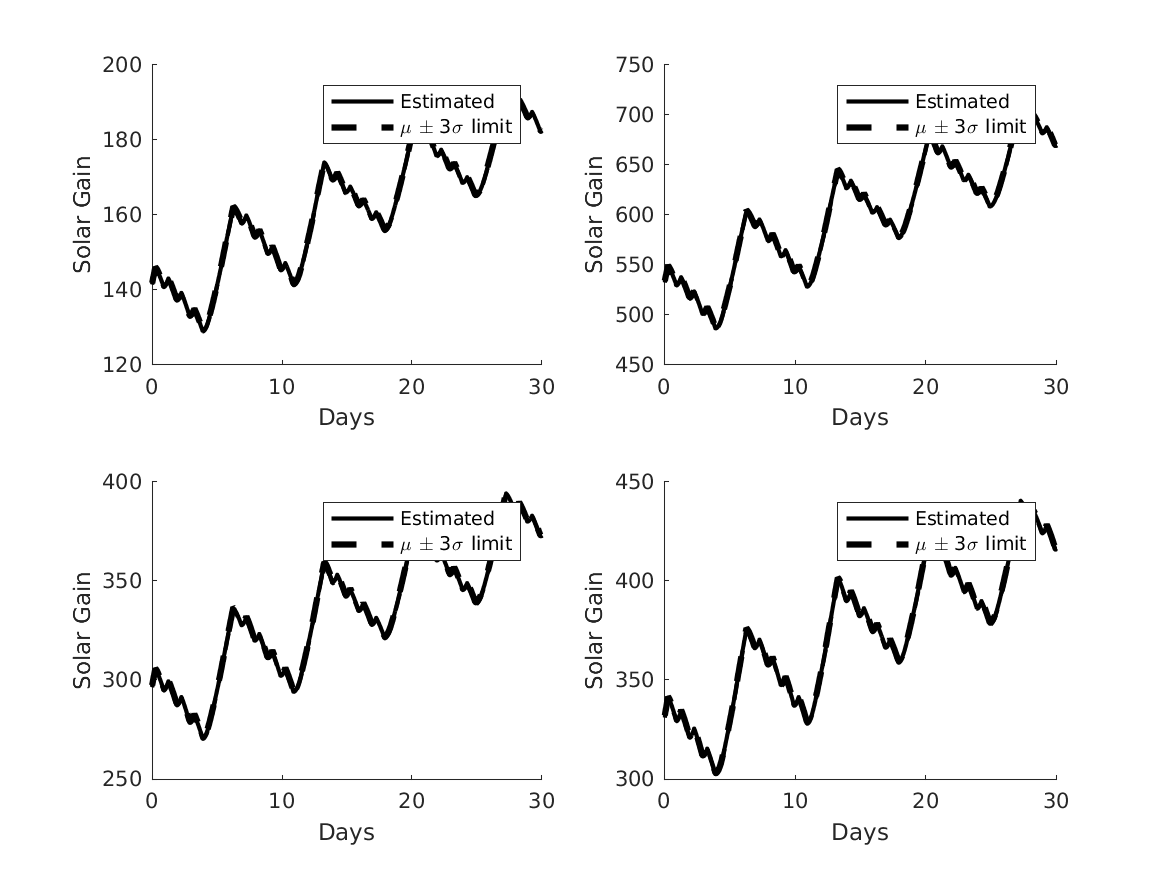
\includegraphics[width=\textwidth]{jbs_figures/solar_2_6}
\caption{Zone 47}
\label{solar_2_6}
\end{subfigure}
\centering
\begin{subfigure}{0.45\textwidth}
\includegraphics[width=\textwidth]{jbs_figures/solar_3_6}
\caption{Zone 97}
\label{solar_3_6}
\end{subfigure} 
\caption{Solar Gains for (a) Zone 47 and (b) Zone 97 for the month of June}
\label{Zone_solar_temperature_june}
\end{figure}

% \begin{figure}[H]
% \centering
% \subfigure[Zone 1]{\includegraphics[width=0.45\textwidth]{figures/solar_2_6}}
% \subfigure[Zone 33]{\includegraphics[width=0.45\textwidth]{figures/solar_3_6}}
% \caption{Solar Gains for (a) Zone 47 and (b) Zone 97 for the month of June}
% \label{Zone_solar_temperature_june}
% \end{figure}

\begin{figure}[H]
\begin{subfigure}{0.45\textwidth}
\centering
\includegraphics[width=\textwidth]{jbs_figures/solar_2_10}
\caption{Zone 47}
\label{solar_2_10}
\end{subfigure}
\centering
\begin{subfigure}{0.45\textwidth}
\includegraphics[width=\textwidth]{jbs_figures/solar_3_10}
\caption{Zone 97}
\label{solar_3_10}
\end{subfigure} 
\caption{Solar Gains for (a) Zone 47 and (b) Zone 97 for the month of October}
\label{Zone_solar_temperature_oct}
\end{figure}

% \begin{figure}[H]
% \centering
% \subfigure[Zone 1]{\includegraphics[width=0.45\textwidth]{figures/solar_2_10}}
% \subfigure[Zone 33]{\includegraphics[width=0.45\textwidth]{figures/solar_3_10}}
% \caption{Solar Gains for (a) Zone 47 and (b) Zone 97 for the month of June}
% \label{Zone_solar_temperature_oct}
% \end{figure}


\section{Summary}
\label{conclusion}

In this chapter, a reduced-order thermal BEM for a large scale office/school building has been developed. The lumped capacitance RC network model is used to calculate the internal load and solar gain. Using the simplified BEM in conjunction with the Weakly Connected Subsystems optimal estimation method allows for estimating internal loads, solar heat gains, and HVAC supply air temperatures.  Furthermore, one can use the outlined framework to calculate the uncertainty of the results \textcolor{red}{for a comprehensive representation} of the building systems.

One significant advantage of the methodology is the ability to reduce the computation expense of large-scale dynamical systems while maintaining accuracy and providing uncertainty information at each step.  Thus, the BEM demonstrated in this work can be built upon, adding detail to offer more precision.  For instance, we included infiltration as part of the internal load estimator; instead, this component could be broken out separately to explore the impact of the envelope leakage on the building model.  

In the same vein, the BEM can be used to compare expected building behavior against the actual building states. This in turn could detect anomalies in the building operation.  Used in conjunction with Model Predictive Control, one can also optimize energy usage and occupant comfort.
The flexibility offered with this technique allows us to vary parameters over time, which is not available in some of the more comprehensive simulation programs.  For example, foam insulation is known to degrade over time, due to the diffusion of thermal gases as the material ages~\citep{de2011longitudinal}.  Most modeling programs, such as eQUEST, require that the thermal conductivity of material remain static over the duration of the simulation.  The conductivity at each time step can be used to provide a more precise representation of the dynamic BEM using the lumped capacitance model.
The technique discussed in this work can be applied to any building and is especially suited for large buildings with diverse occupancy, due to the inter-zone effects, and variable internal loads. With the noise filtered out and the zonal temperatures being estimated, the solar gains and the internal loads can be checked. 













